\documentclass{standalone}
\usepackage{tikz}
\usetikzlibrary{patterns, positioning}
\usepackage[sfdefault]{ClearSans} %% option 'sfdefault' activates Clear Sans as the default text font
\usepackage[T1]{fontenc}

\begin{document}
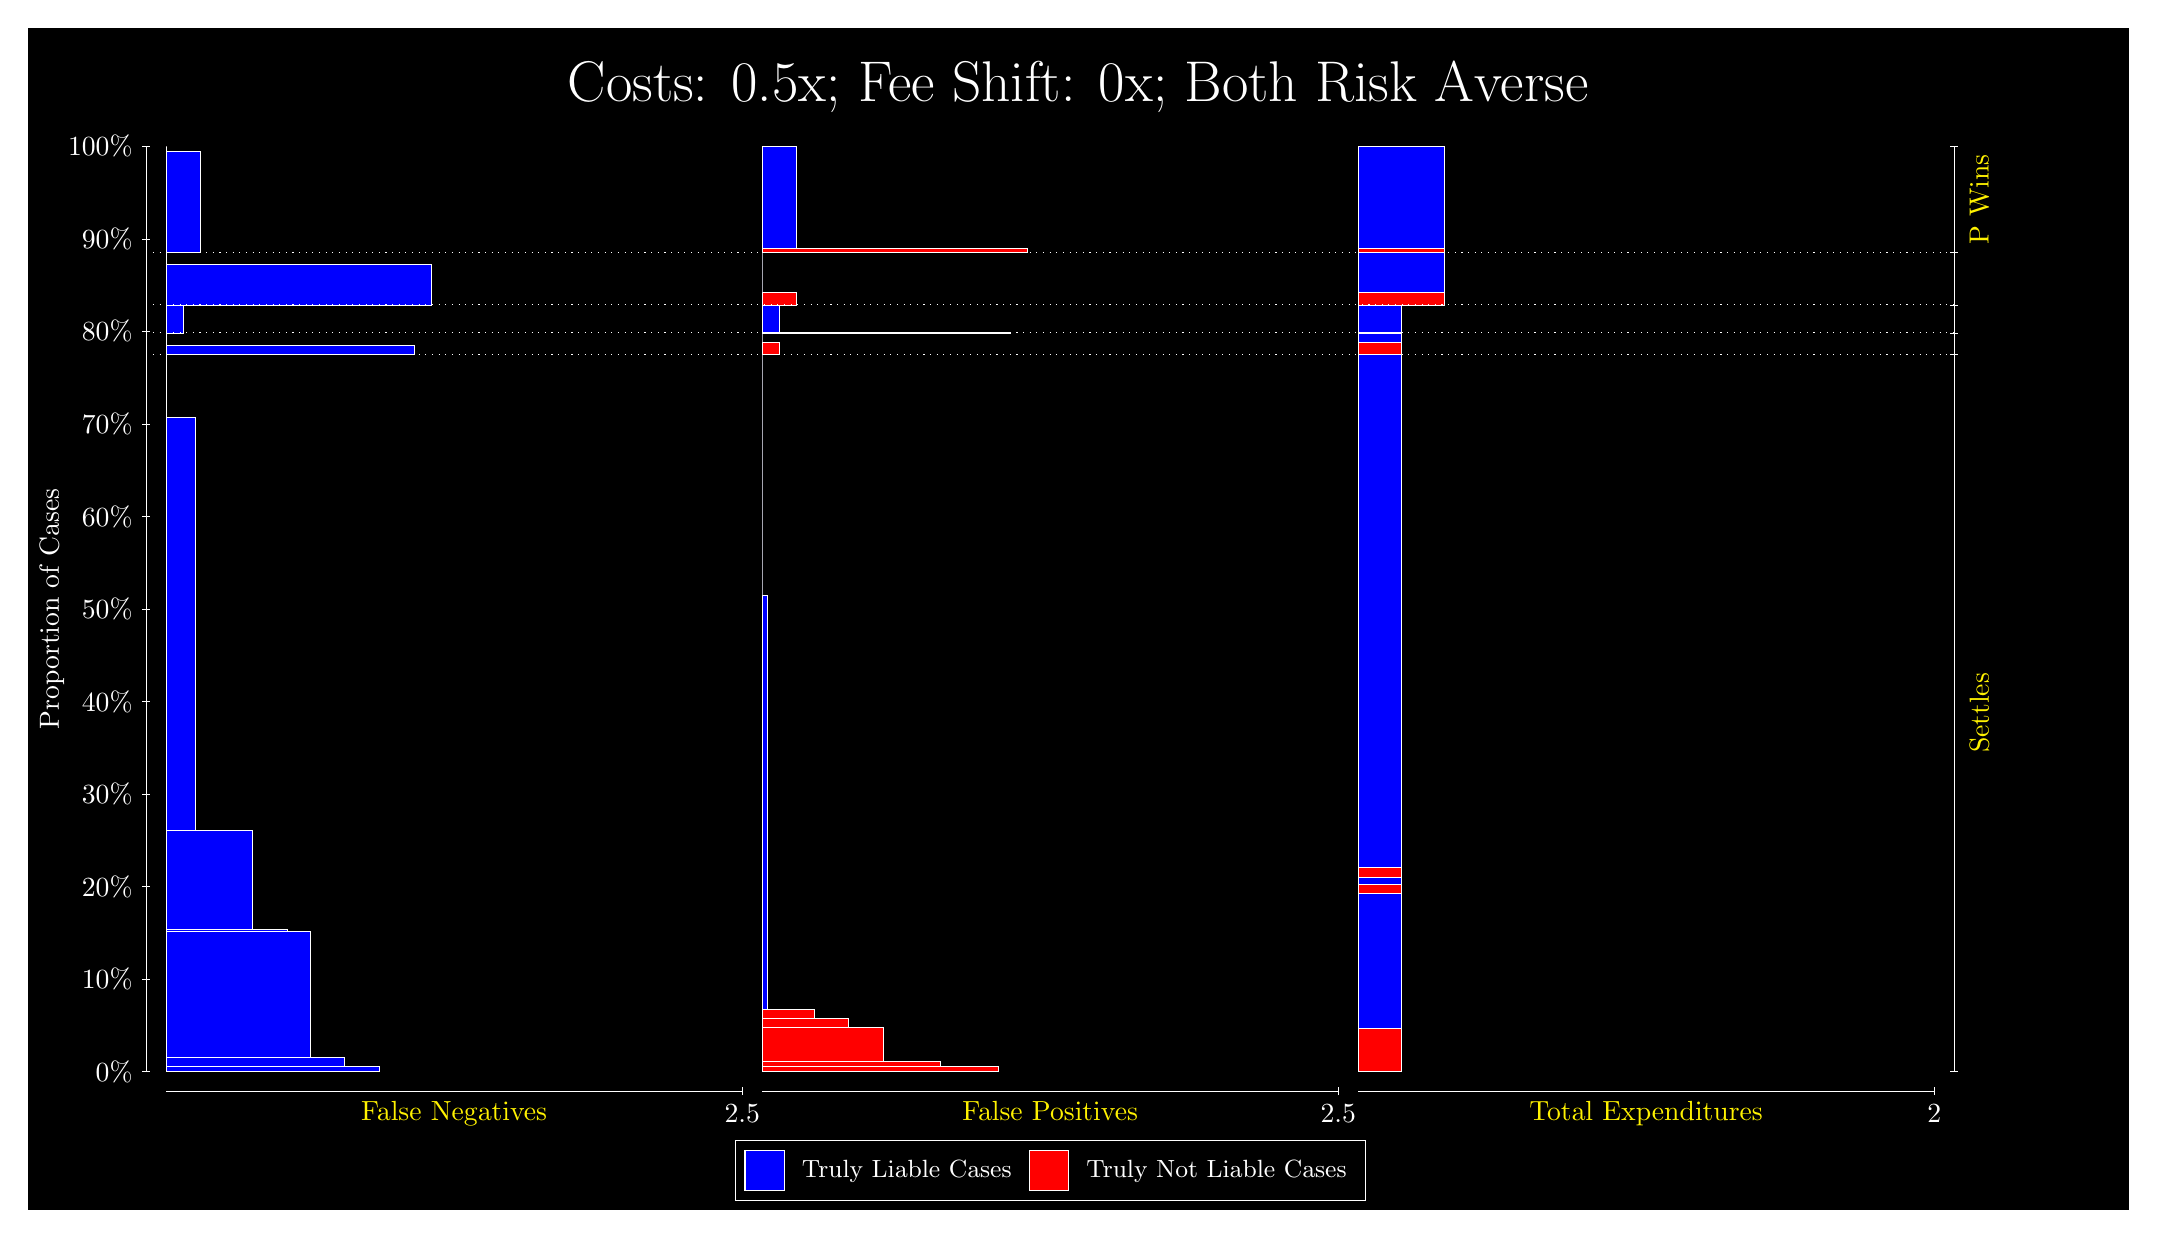
\begin{tikzpicture}
\draw[fill=black] (0,0) rectangle (26.667,15);
\draw[text=white] (0,13.5) rectangle (26.667,15) node[midway] {\huge Costs: 0.5x; Fee Shift: 0x; Both Risk Averse};
\draw[white, very thin] (1.5,1.75) -- (1.5,13.5);
\node[rotate=90, text=white, anchor=center] at (0.3, 7.625) {Proportion of Cases};
\draw[white, very thin] (1.45,1.75) -- (1.55,1.75);
\node[text=white, anchor=east] at (1.45, 1.75) {0\%};
\draw[white, very thin] (1.45,2.925) -- (1.55,2.925);
\node[text=white, anchor=east] at (1.45, 2.925) {10\%};
\draw[white, very thin] (1.45,4.1) -- (1.55,4.1);
\node[text=white, anchor=east] at (1.45, 4.1) {20\%};
\draw[white, very thin] (1.45,5.275) -- (1.55,5.275);
\node[text=white, anchor=east] at (1.45, 5.275) {30\%};
\draw[white, very thin] (1.45,6.45) -- (1.55,6.45);
\node[text=white, anchor=east] at (1.45, 6.45) {40\%};
\draw[white, very thin] (1.45,7.625) -- (1.55,7.625);
\node[text=white, anchor=east] at (1.45, 7.625) {50\%};
\draw[white, very thin] (1.45,8.8) -- (1.55,8.8);
\node[text=white, anchor=east] at (1.45, 8.8) {60\%};
\draw[white, very thin] (1.45,9.975) -- (1.55,9.975);
\node[text=white, anchor=east] at (1.45, 9.975) {70\%};
\draw[white, very thin] (1.45,11.15) -- (1.55,11.15);
\node[text=white, anchor=east] at (1.45, 11.15) {80\%};
\draw[white, very thin] (1.45,12.325) -- (1.55,12.325);
\node[text=white, anchor=east] at (1.45, 12.325) {90\%};
\draw[white, very thin] (1.45,13.5) -- (1.55,13.5);
\node[text=white, anchor=east] at (1.45, 13.5) {100\%};

\draw[white, very thin] (24.457,1.75) -- (24.457,13.5);
\draw[white, very thin] (24.407,1.75) -- (24.507,1.75);
\node[anchor=west] at (24.407, 1.75) {};
\draw[white, very thin] (24.407,10.859) -- (24.507,10.859);
\node[anchor=west] at (24.407, 10.859) {};
\draw[white, very thin] (24.407,11.132) -- (24.507,11.132);
\node[anchor=west] at (24.407, 11.132) {};
\draw[white, very thin] (24.407,11.486) -- (24.507,11.486);
\node[anchor=west] at (24.407, 11.486) {};
\draw[white, very thin] (24.407,12.154) -- (24.507,12.154);
\node[anchor=west] at (24.407, 12.154) {};
\draw[white, very thin] (24.407,13.5) -- (24.507,13.5);
\node[anchor=west] at (24.407, 13.5) {};

\draw[white, very thin, fill=blue] (1.75,1.75) rectangle (4.458,1.8107);
\draw[white, very thin, fill=blue] (1.75,1.8107) rectangle (4.0188,1.9334);
\draw[white, very thin, fill=blue] (1.75,1.9334) rectangle (3.5797,3.5283);
\draw[white, very thin, fill=blue] (1.75,3.5283) rectangle (3.287,3.5515);
\draw[white, very thin, fill=blue] (1.75,3.5515) rectangle (2.8478,4.8162);
\draw[white, very thin, fill=blue] (1.75,4.8162) rectangle (2.1159,10.063);
\draw[white, very thin, fill=red] (1.75,10.063) rectangle (1.75,10.859);
\draw[white, very thin, fill=blue] (1.75,10.859) rectangle (4.8971,10.974);
\draw[white, very thin, fill=red] (1.75,10.974) rectangle (1.75,11.132);
\draw[white, very thin, fill=blue] (1.75,11.132) rectangle (1.9696,11.479);
\draw[white, very thin, fill=red] (1.75,11.479) rectangle (1.75,11.486);
\draw[white, very thin, fill=blue] (1.75,11.486) rectangle (5.1167,11.998);
\draw[white, very thin, fill=red] (1.75,11.998) rectangle (1.75,12.154);
\draw[white, very thin, fill=blue] (1.75,12.154) rectangle (2.1891,13.443);
\draw[white, very thin, fill=red] (1.75,13.443) rectangle (1.75,13.5);
\draw[white, very thin, fill=red] (9.3189,1.75) rectangle (12.32,1.8155);
\draw[white, very thin, fill=red] (9.3189,1.8155) rectangle (11.588,1.881);
\draw[white, very thin, fill=red] (9.3189,1.881) rectangle (11.149,1.8865);
\draw[white, very thin, fill=red] (9.3189,1.8865) rectangle (10.856,2.3161);
\draw[white, very thin, fill=red] (9.3189,2.3161) rectangle (10.417,2.4298);
\draw[white, very thin, fill=red] (9.3189,2.4298) rectangle (9.9776,2.5464);
\draw[white, very thin, fill=blue] (9.3189,2.5464) rectangle (9.3921,7.7929);
\draw[white, very thin, fill=blue] (9.3189,7.7929) rectangle (9.3189,10.859);
\draw[white, very thin, fill=red] (9.3189,10.859) rectangle (9.5384,11.017);
\draw[white, very thin, fill=blue] (9.3189,11.017) rectangle (9.3189,11.132);
\draw[white, very thin, fill=red] (9.3189,11.132) rectangle (12.466,11.139);
\draw[white, very thin, fill=blue] (9.3189,11.139) rectangle (9.5384,11.486);
\draw[white, very thin, fill=red] (9.3189,11.486) rectangle (9.758,11.642);
\draw[white, very thin, fill=blue] (9.3189,11.642) rectangle (9.3189,12.154);
\draw[white, very thin, fill=red] (9.3189,12.154) rectangle (12.686,12.211);
\draw[white, very thin, fill=blue] (9.3189,12.211) rectangle (9.758,13.5);
\draw[white, very thin, fill=red] (16.888,1.75) rectangle (17.437,2.2932);
\draw[white, very thin, fill=blue] (16.888,2.2932) rectangle (17.437,4.0108);
\draw[white, very thin, fill=red] (16.888,4.0108) rectangle (17.437,4.133);
\draw[white, very thin, fill=blue] (16.888,4.133) rectangle (17.437,4.2169);
\draw[white, very thin, fill=red] (16.888,4.2169) rectangle (17.437,4.3479);
\draw[white, very thin, fill=blue] (16.888,4.3479) rectangle (17.437,10.859);
\draw[white, very thin, fill=red] (16.888,10.859) rectangle (17.437,11.017);
\draw[white, very thin, fill=blue] (16.888,11.017) rectangle (17.437,11.132);
\draw[white, very thin, fill=red] (16.888,11.132) rectangle (17.437,11.139);
\draw[white, very thin, fill=blue] (16.888,11.139) rectangle (17.437,11.486);
\draw[white, very thin, fill=red] (16.888,11.486) rectangle (17.986,11.642);
\draw[white, very thin, fill=blue] (16.888,11.642) rectangle (17.986,12.154);
\draw[white, very thin, fill=red] (16.888,12.154) rectangle (17.986,12.211);
\draw[white, very thin, fill=blue] (16.888,12.211) rectangle (17.986,13.5);
\draw[white, dotted] (1.5,10.859) -- (24.457,10.859);
\draw[white, dotted] (1.5,11.132) -- (24.457,11.132);
\draw[white, dotted] (1.5,11.486) -- (24.457,11.486);
\draw[white, dotted] (1.5,12.154) -- (24.457,12.154);
\draw[white, very thin] (1.75,1.5) -- (9.0689,1.5);
\node[text=yellow, anchor=north] at (5.4094, 1.5) {False Negatives};
\draw[white, very thin] (9.0689,1.45) -- (9.0689,1.55);
\node[text=white, anchor=north] at (9.0689, 1.45) {2.5};

\draw[white, very thin] (9.3189,1.5) -- (16.638,1.5);
\node[text=yellow, anchor=north] at (12.978, 1.5) {False Positives};
\draw[white, very thin] (16.638,1.45) -- (16.638,1.55);
\node[text=white, anchor=north] at (16.638, 1.45) {2.5};

\draw[white, very thin] (16.888,1.5) -- (24.207,1.5);
\node[text=yellow, anchor=north] at (20.547, 1.5) {Total Expenditures};
\draw[white, very thin] (24.207,1.45) -- (24.207,1.55);
\node[text=white, anchor=north] at (24.207, 1.45) {2};

\node[text=yellow, centered, rotate=90] at (24.777, 6.3046) {Settles};



\node[text=yellow, centered, rotate=90] at (24.777, 12.827) {P Wins};

\draw (12.978300999999998,1.5) node[draw=none] (baseCoordinate) {};
\begin{scope}[align=center]
        \matrix[scale=0.5, draw=white, below=0.5cm of baseCoordinate, nodes={draw}, column sep=0.1cm]{
            \node[rectangle, draw, minimum width=0.5cm, minimum height=0.5cm, fill=blue] {}; &
            \node[draw=none, font=\small, text=white] (B) {Truly Liable Cases}; &
            \node[rectangle, draw, minimum width=0.5cm, minimum height=0.5cm, fill=red] {}; &
            \node[draw=none, font=\small, text=white] (B) {Truly Not Liable Cases}; \\
            };
\end{scope}

\end{tikzpicture}
\end{document}